\section{Execution Plan}
\label{executionplan}

The general execution pipeline, in figure \ref{pipeline}, provides an overview of the steps that have been followed. Hereafter, we will analyse for each research question how the experiment was conducted.
\subsection{\textbf{RQ$_{1}$} - Comparing a standard ViT with Our Proposal} 
After implementing in PyTorch our architecture described in  section \ref{architecture} we are going to train from scratch a ViT and our model and comparing them using the metrics explained in section \ref{metrics}.
For the energy efficiency analysis we will use CodeCarbon, which provides an accurate estimation of the energy producted by RAM, GPUs and CPUs during the executing of the code (we will use Colab to perform the operations in as isolated an environment as possible \textit{"Intel Xeon @ 2.20GHz and Tesla T4 GPU"}). 

We will perform a statistical validity test with null hypothesis stating that the sample (Electric energy consumed repeating the same experiment) follows a normal PDF and alternative hypothesis stating that it does not come from that distribution:
\begin{itemize}
    \item We will perform the Shapiro-Wilk test with significance level 0.05 in the hope of validating the null hypothesis 
    \item If the tests confirm the null hypothesis, then the energy values we will report will be the average of the calculated values.
    \item Finally, we will calculate the Carbon Intensity, which is the grams of CO$_2$ produced by running the code as the product of the Net Carbon Intensity (A weighted average of the emissions from the different energy sources that are used to generate electricity consumed by the Cloud provider or Country) and the KWh consumed.
\end{itemize}

\subsection{\textbf{RQ$_{2}$} - In Search of Heuristic that lead to a faster convergence}
When a human being is asked to understand an object represented on an image, a logical process is generally carried out that leads to discarding all information that does not concern the object itself. Based on this theory, we will implement a feature selection layer based on three different heuristics.
Given that every patch in which the image is divided is an $n \times n$ matrix the value of each patch $x$ is calculated as follows:
\begin{itemize}
    \item Contrast (Figure \ref{fig:dog_contrast}):  $$F(x) =  \frac{max(x) - min(x) + 10^{-8}}{max(x) + min(x)}$$ 
   
    \item Variance (Figure \ref{fig:dog_variance}): $$F(x) =  \frac{\sum_{i=1}^n\left(x_i-\overline{\mathbf{x}}\right)^2}{n-1}$$
       
    \item Entropy (Figure \ref{fig:dog_entropy}): $$F(x) =  -\sum_{i=1}^{n}(p_i * log2(p_i))$$\\ where $$p_i = \frac{count(i)}{N}$$
        
\end{itemize}
    \begin{figure}[!htp]
        \centering
        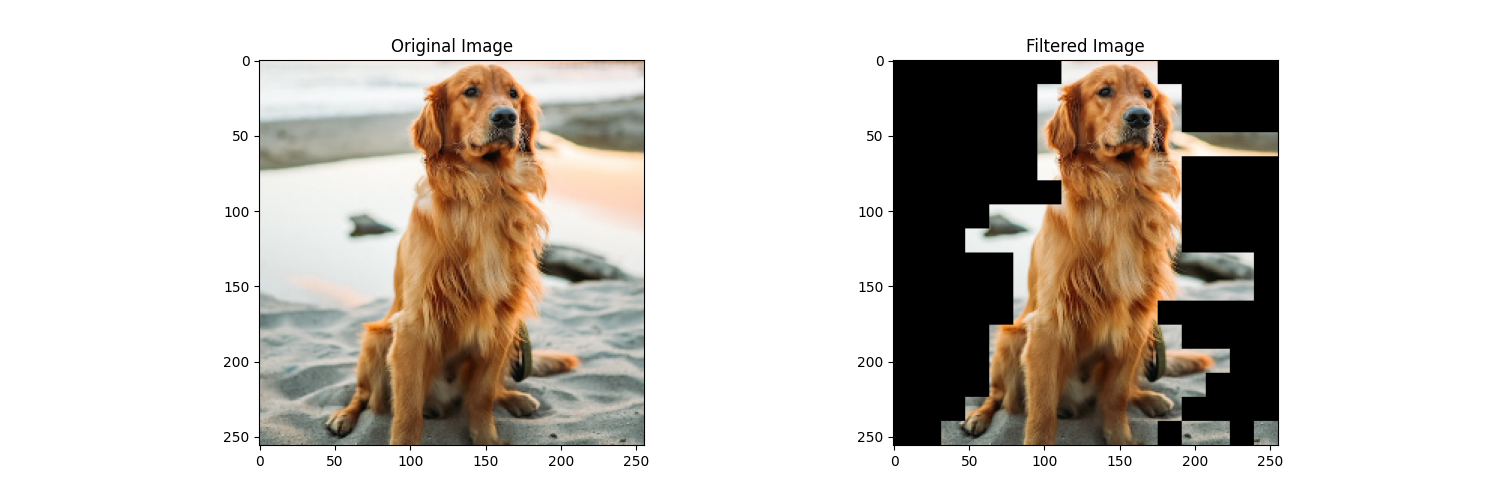
\includegraphics[width=\columnwidth]{images/dog_contrast.png}
        \caption{Image filtered based on contrast values distribution preserving 50\% of image}
        \label{fig:dog_contrast}
    \end{figure}
     \begin{figure}[!htp]
        \centering
        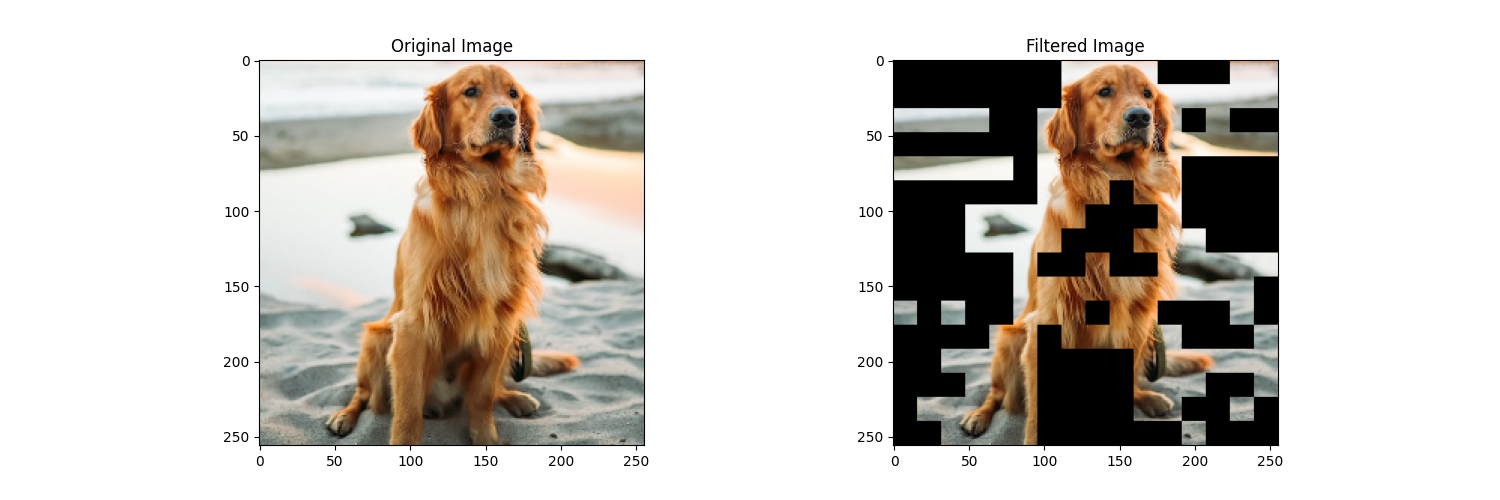
\includegraphics[width=\columnwidth]{images/dog_variance.png}
        \caption{Image filtered based on variance values distribution preserving 50\% of image}
        \label{fig:dog_variance}
    \end{figure}
    \begin{figure}[!htp]
        \centering
        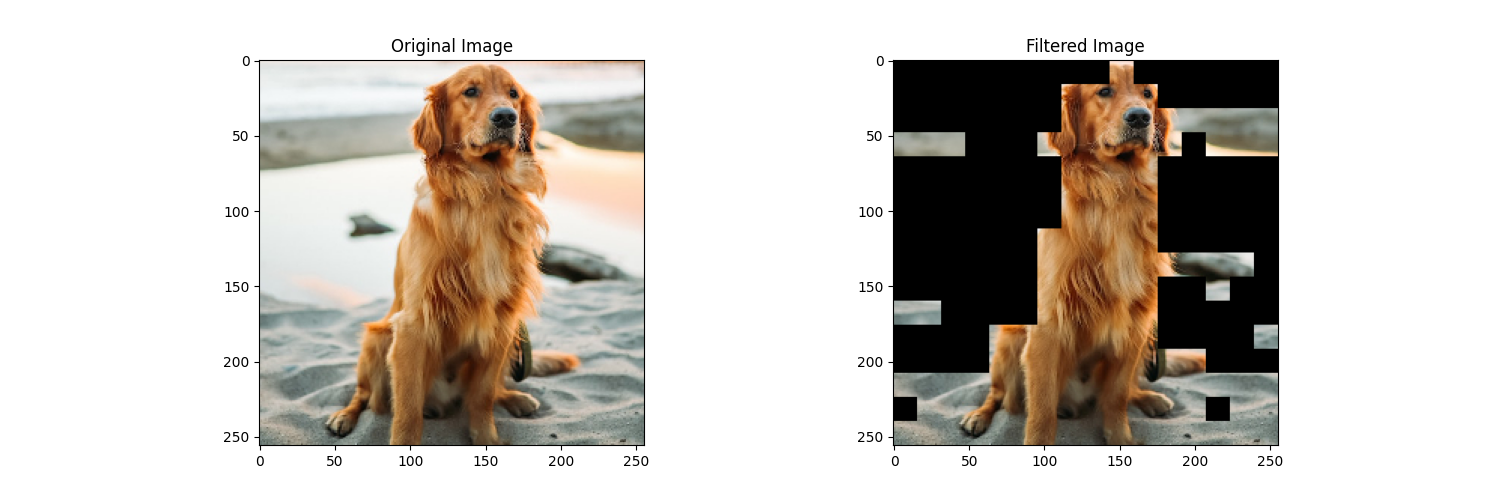
\includegraphics[width=\columnwidth]{images/dog_entropy.png}
        \caption{Image filtered based on contrast entropy distribution preserving 50\% of image}
        \label{fig:dog_entropy}
    \end{figure}
\subsection{\textbf{RQ$_{3}$} - Assessing the Performance of Our Model on different training technique} In this phase we will train our model using two different techniques

1) Pre-training + Fine-tuning

2) Pre-training + Contrastive Learning + Fine-tuning
\\
Each phase will be executed as follows:
\begin{itemize}
    \item Pre-training: the model will be trained on a large amount of unlabeled data to learn general features. In our pre-training, the model is trained on ImageNet using a self-supervised task called 'masked language modeling.' This involves randomly masking some patches of the input image and then training the model to predict the masked patches. This way, the model learns to represent the image in terms of meaningful patches of varying sizes and positions.

    \item Contrastive Learning: after pre-training, the model will be further fine-tuned using contrastive learning, which is a form of self-supervised learning. In contrastive learning, the model learns to distinguish between similar and dissimilar image patches by projecting them into a high-dimensional space and comparing their distances. This way, the model learns to identify patterns and features that are relevant for the downstream task, such as image recognition.

    \item Fine-tuning: once the model has been pre-trained and fine-tuned with contrastive learning, it will be further fine-tuned onimage recognition task on CIFAR-10/CIFAR-100. During fine-tuning, the model is trained on labeled data with a supervised learning approach. In this phase, the last few layers of the model are replaced with new ones, and only the newly added layers are trained on the specific task, while the earlier layers are frozen to retain the learned features. This way, the model can adapt to the specific dataset and learn to recognize the relevant features for the task at hand.
\end{itemize}